% !TeX encoding = UTF-8
\section{Umsetzung}
\label{sec:Umsetzung}
Bevor wir uns den notwendigen Anpassungen des \textit{RRT*}-Algorithmus widmen können, müssen wir die kinematischen und physikalischen Beschränkungen des Autos analysieren. Anschließend wird das verwendete Framework ROS - Robot Operating Systems - vorgestellt, wonach wir uns mit der Wahl einer geeigneten Metrik und Kostenfunktion beschäftigen.
\subsection{Hardwareausstattung der Autos}
Das Dahlem Center for Machine Learning and Robotics arbeitet mittlerweile mit dem Modelfahrzeug AutoNOMOS Mini v3 (1:10).[TODO Bild anfügen] Der Hauptcomputer auf dem Auto ist ein \textit{Odroid}(XU4 64GB) mit Ubuntu Linux als Betriebssystem und ROS (Robot Operation Systems) als Steuerungssystem \citep{fubAuto}.\\
\begin{figure}
\centering
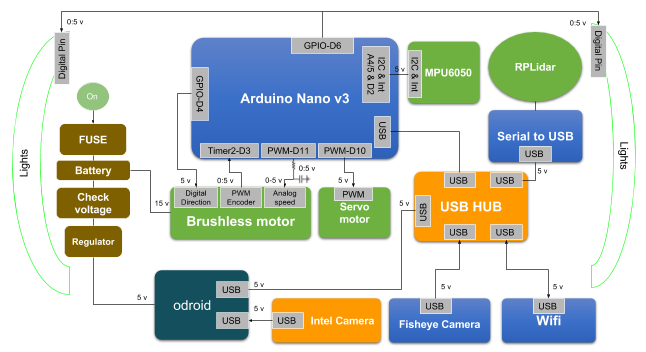
\includegraphics[scale=0.8]{Bilder/AutoNOMOS_mini_v3.png} 
\caption{Überblick über die Module des AutoNOMOS Mini v3}
\end{figure}
Motorisiert ist das Auto mit einem bürstenlosen [TODO??] DC-Servomotor FAULHABER 2232. Die Lenkung wird von dem Servomotor HS-645-MG übernommen, beide Motoren werden mithilfe einer \textit{Arduino Nano} Platine gesteuert. \\
Zur Wahrnehmung der Umgebung besitzt das AutoNOMOS Mini v3 mit dem RPLIDAR A2 360 einen rotierenden Laserscanner, der in der Lage ist, die Umgebung des Autos auf Hindernisse zu überprüfen. Als Rückgabewert liefert der RPLIDAR pro Gradwinkel den Wert, wie weit das nächste Hindernis in dieser Richtung entfernt ist, also insgesamt 360 Werte (einen pro Winkel). \\
Auf dem oberen Teil des Autos befestigt ist das \textit{Kinect-type stereoscopic system} (Intel RealSense SR300), welches eine Wolke aus 3D Punkten liefert, die dazu benutzt werden kann, Hindernisse zu erkennen. Außerdem kann die Kamera des \textit{Kinect-type} Sensors dazu benutzt werden, Fahrbahnmarkierungen und Objekte direkt vor dem Auto zu lokalisieren.\\
Der letzte äußere Sensor, auch am oberen Teil des Autos angebracht, ist die Fischaugen-Kamera. Diese zeigt nach oben, zur Decke, und kann dazu benutzt werden bestimmte markante, feststehende Objekte zu lokalisieren, damit das AutoNOMOS Mini v3 sich auch innerhalb von Räumen orientieren kann. Dazu kann eine GPS Navigationseinheit simuliert werden, indem die an der Decke angebrachten vier Lampen in unterschiedlichen Farben leuchten. \\
Die Sensoren sind entweder via USB 3.0 an der Hauptplatine oder direkt am \textit{Odroid} angeschlossen. \\
An inneren Sensoren besitzt das AutoNOMOS Mini v3 eine MPU6050, die einen Beschleunigungssensor und ein \textit{Gyroskop} enthält. Mithilfe dieser MPU kann das AutoNOMOS Mini v3 seine Orientierung, seine Richtung im Raum bestimmen. Außerdem können Messungen zur \textit{Odometrie} ergänzt werden.\\
Das AutoNOMOS Mini v3 wird über eine 14,8 V Batterie mit Energie versorgt.

\subsection{Software: ROS - Robot Operating Systems}
ROS stellt Bibliotheken und Werkzeuge zur Verfügung, die Software-Entwicklern helfen sollen, Robotik Anwendungen zu kreieren \citep{ROS}. Unter anderem beinhaltet ROS Gerätetreiber, Bibliotheken, Visualisierungswerkzeuge, Paketmanagement und vieles mehr. ROS ist Open Source und unter der BSD Lizenz verfügbar.
\subsubsection{Architektur}
Mithilfe von ROS können so genannte \textit{Nodes}, ausführbare Programme, erzeugt werden, die über so genannte \textit{Topics} kommunizieren können. Dies passiert über einen anonymisierten Publisher/Subscriber Mechanismus, das heißt Daten generierende Knoten können auf relevanten \textit{Topics} Nachrichten senden, und interessierte Knoten können von relevanten \textit{Topics} Nachrichten empfangen. \\
Für jedes \textit{Topic} ist dabei auch die Nachrichtenart definiert, die für dieses \textit{Topic} veröffentlicht und von diesem \textit{Topic} empfangen werden. Dies können neben simplen Datentypen auch komplexe, selbst definierte Datenstrukturen sein. Dabei wird nur dieser eine, vorher festgelegte Datentyp der Nachricht vom \textit{Topic} akzeptiert.
\textit{Topics} stellen nur eine unidirektionale Verbindung zur Verfügung. Für die Abwicklung von zum Beispiel Remote Procedure Calls sind sogenannte Services zuständig. Diese ermöglichen, eine Antwort auf eine bestimmte Anfrage nach dem Client Server Prinzip zurückzusenden.
\subsection{APIs und Einbettung zu bereits vorhandene Knoten}
Das Dahlem Center for Machine Learning and Robotics entwickelte ROS-Pakete für die Steuerung ihrer autonomer Fahrzeuge. Diese Pakete und daraus resultierenden ROS-Nodes können dazu genutzt werden, den von mir entwickelten RRT*-Pfadplaner möglichst gut einzubetten. So kann durch das visuelle indoor GPS die Position des Autos bestimmt werden, die der Pfadplaner für seine Berechnungen braucht. Die resultierende \textit{Trajektorie}, die der Pfadplaner entwickelt, wird einem Steuerungsknoten übergeben, der diese \textit{Trajektorie} in Motorbefehle, also Beschleunigungen und Lenkungen, umsetzt. 
\subsubsection{Bestimmung der Odometry und visual GPS}
[TODO was benutzte ich jetzt?]

\subsubsection{Steuerungsknoten fubController}
Dieser Knoten lauscht auf das \textit{Topic} \verb|"planned_path"|. Auf \verb|"planned_path"| kann eine \textit{Trajektorie} publiziert werden, die dann mithilfe des Steuerungsknotens vom Auto abgefahren wird. Dabei kümmert sich dieser Steuerungsknoten allerdings nicht um etwagige Hindernisse, die mit dem Auto kollidieren könnten. Somit muss der Pfadplaner selbst alle Kollisionen mit Hindernissen ausschließen. \\
Das Format der \textit{Trajektorie} wurde von der Arbeitsgruppe der FU Berlin definiert und besteht aus
\begin{itemize}
\item \verb|std_msgs/Header|: Hier wird die aktuelle Zeit gespeichert.
\item \verb|string child_frame_id|: [TODO]
\item \verb|fub_trajectory_msgs/TrajectoryPoint[] trajectory|: Eine Liste aus Trajektorie-Punkten.
\end{itemize}
Ein Trajektorien-Punkt symbolisiert einen abzufahrenden Knotenpunkt und wiederum besteht aus
\begin{itemize}
\item \verb|geometry_msgs/Pose pose|: Hier sind Position und Orientierung des Autos gespeichert.
\item \verb|geometry_msgs/Twist velocity|:Hier wird die Geschwindigkeit des Autos an diesem Punkt gespeichert.
\item \verb|geometry_msgs/Twist acceleration| Hier wird die Beschleunigung des Autos an diesem Punkt gespeichert.
\end{itemize}
Die Position wird in x-Position und y-Position angegeben, ausgehend von einer Ecke des Raumes. Die Orientierung wird durch ein \textit{Quaternion} dargestellt, bei dem durch vier Werte die Drehung in jeder Richtung des Raumes genau bestimmt ist. Allerdings genügt uns die Drehung um die z-Achse, also die Drehrichtung über die Vertikalachse, weshalb dieses Quaternion in einen Winkel, der sogenannten Gierung, umgerechnet wird.
\\
Nachdem die notwendige Infrastruktur erläutert wurde, folgt eine kurze Betrachtung der kinematischen und physikalischen Einschränkungen, denen das AutoNOMOS Mini v3 unterworfen ist. Anschließend können wir uns endlich dem Kernstück der Arbeit, dem eigentlichen RRT*-Pfadplaner, widmen.

\subsection{Kinematische und physikalische Einschränkungen}
Im Gegensatz zu holonomischen Fahrzeugen sind die möglichen Pfade eines Autos nicht so einfach zu berechnen. Deshalb stellen wir zuerst zur Orientierung ein mathematisches Modell des Autos auf und definieren die Randbedingungen, unter denen es agiert.
Die mathematischen Definitionen der Randbedingungen und des Autos sind in der Bachelorarbeit von Lukas Gödicke \citep{Goedicke18} gut beschrieben und werden hier (übersetzt) übernommen. \\
\subsubsection{Randbedingungen}
Die Position des Autos bezieht sich auf den Mittelpunkt zwischen den Hinterrädern mit den Koordinaten x und y. Der Winkel $\theta \in S,  S=[0,2\pi]$ steht für die Ausrichtung des Autos, der Winkel $\phi \in S$ für die Ausrichtung der Räder (=Lenkwinkel). Wir nehmen an, dass das Auto sich auf einer flachen Ebene bewegt. Somit ist der Arbeitsraum definiert durch $C =  \mathbb{R \times S}$. Ein Zustand des Autos wird beschrieben durch $q \in C = (x,y,\theta)$.\\
Zur Vereinfachung der Rechnungen wird angenommen, dass die Räder bei Bedarf sich sofort, ohne Zeitverlust, in die gewünschte Position begeben. Da der Lenkwinkel keinen Einfluss auf den Momentanzustand des Autos hat wird dieser in der Zustandsbeschreibung nicht aufgeführt. Zusätzlich kommt noch hinzu, dass das Auto zur Testzwecken bestimmte Geschwindigkeiten nicht überschreiten darf, sodass der minimale Kurvenradius nur durch den Lenkwinkel beschränkt ist und nicht auch noch zusätzlich durch die Geschwindigkeit. \\

\subsubsection{Einschränkungen durch das Auto}
Ein Auto hat eine Möglichkeit sich fortzubewegen: Es kann beschleunigen. Eine negative Beschleunigung wäre Bremsen oder sogar Rückwärtsfahren. Zusätzlich zu dieser einen Möglichkeit, den Zustand des Autos zu ändern, kann das Auto das Resultat der Beschleunigung ändern, indem der Lenkwinkel angepasst wird. Dieser reicht von $\phi_{max}$ bis $-\phi_{max}$, den maximalen Lenkwinkeln des Autos.
Je nach Lenkwinkel $i_{\phi}$, Geschwindigkeit $i_g$ und Anfangsausrichtung des Autos $\theta$ ändern sich verschiedene Parameter des Zustandes $q(x,y, \theta) $: \\
\begin{center}
$ \dot{x} = i_g cos \phi $ \\
$ \dot{y} = i_g sin \phi$ \\
$ \dot{{\theta}} = \frac{i_g}{L} tan (i_{\phi}) $
\end{center}
L ist hierbei der Radstand, also der Abstand zwischen Vorder- und Hinterachse.

\subsubsection{Konsequenzen}
Ein normaler \textit{RRT*} besitzt \textit{Trajektorien} zum Ziel, die für ein Auto aufgrund der oben benannten Beschränkungen nicht abfahrbar sind. So entstehen beispielsweise diskrete Ecken und Kanten die für ein sich kontinuierlich bewegendes Auto unmöglich zu bewältigen ist. Somit ist die erste Aufgabe, die Pfade im \textit{RRT*} für das Auto irgendwie abfahrbar zu machen.\\
Dazu hatte ich am Anfang unterschiedliche Ansätze:
\begin{enumerate}
\item RRT* normal ausführen. Sobald ein Pfad zum Ziel gefunden: Diesen so bearbeiten, dass dieser vom Auto zu bewältigen ist
\item RRT* normal ausführen, jedoch mit geeignetem Algorithmus dafür sorgen, dass das Auto jeden Knoten erreichen kann
\item Nur Knoten hinzufügen, die von ihrem Vaterknoten aus unter oben genannten Bedingungen stets erreichbar sind
\end{enumerate}
Das Problem des ersten Ansatzes war, das unter Umständen je nach Umgebung ein Pfad nicht nur wegen bestimmter Ecken und Kanten nicht abfahrbar ist, sondern auch wegen Kurven, die Aufgrund des Lenkradius des Autos nicht zu bewältigen wären. Es wäre zwar möglich, für kurze Zeit die geplante Trajektorie zu verlassen und nach Ende der Kurve wieder zu ihr zu stoßen, allerdings ist es unter diesen Umständen schwierig eine Hindernisfreiheit zu garantieren. \\
Die zweite Variante war Thema der Bachelorarbeit meines oben bereits erwähnten Kommolitonen David Gödicke \citep{Goedicke18}. Dieser benutze für den Pfad zwischen zwei Kurven Dubins Curves \citep{Dubin61}, bei denen drei Einstellungen aus linkem maximalem Lenkeinschlag, rechtem maximalen Lenkeinschlag und geradeaus fahren dreimal hintereinander verkettet werden . Damit kann zwar jeder Punkt des Arbeitsbereiches erreicht werden, allerdings war die Berechnung zu aufwändig und langsam, was für Echtzeit Szenarien im Straßenverkehr ein hartes Ausschlusskriterium ist \citep[vergleiche][Kapitel 7]{Goedicke18}. \\
Deshalb entschloss ich mich für die dritte Variante, bei der Knoten nur zum RRT*-Graph unter der Bedingung hinzugefügt werden, dass sie erreichbar sind.

\subsection{RRT*-Pfadplaner für autonome Fahrzeuge}
\subsubsection{Vorauswahl}
\label{sec:Vorauswahl}
Diese beinhaltete, bei der Erstellung des RRT* vom Auto nicht erreichbare Knoten gar nicht erst zuzulassen. Das Auto sollte also von einem Knoten zum nächsten mit nur einer Lenkeinstellung direkt fahren können. Dies sollte die Berechnungszeit stark verringern. \\
Zum Ausschluss der Knoten verwendete ich zuerst eine Heuristik: Ein nächster Nachbar N für einen neu hinzugefügten Knoten K kam nur dann in Frage, falls dieser den neu hinzugefügten Knoten K auch erreichen konnte. Dazu wurde die Ausrichtung des Autos im potenziellen Elternknoten N mit dem Richtungsvektor zwischen den beiden Knoten verglichen. Somit war K gültig, falls der Winkel zwischen der Ausrichtung von N und dem direktem Weg zum Knoten K (Richtungsvektor) einen bestimmten Wert $\gamma$ nicht überschritt.
\begin{figure}
\centering
\label{fig:fig4}
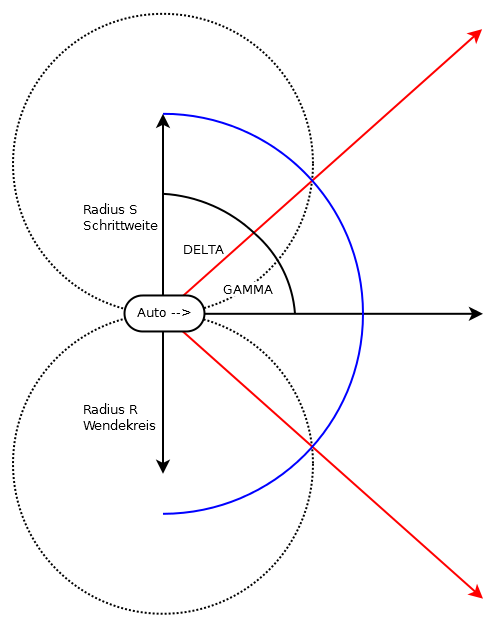
\includegraphics[scale=0.6]{Bilder/AusrichtungGrob.png} 
\caption{Bedeutung der Schrittweite und Radius für den Winkel Gamma}
\end{figure}
 $\gamma$ direkt zu berechnen war nicht ohne weiteres möglich, doch mit Hilfe des Kosinussatzes konnte der Winkel $\delta$ (siehe Abbildung ~\ref{fig:fig4}) berechnet werden. Dieser berechnet sich aus dem Radius $R$ des Wendekreises des Autos und der verwendeten Schrittweite, also dem maximalen Abstand zwischen zwei Knoten. \\
Der Knoten K konnte wurde im ersten Schritt als gültig erkannt, wenn für die Differenz zum Winkel des Elternknoten galt: 
\begin{center}
$diff(K,N) <\gamma$ \\
$\gamma = 90^{\circ} - \delta$  \\
$\delta = arccos (\frac{Schrittweite}{2 \dot R})$  \\
\end{center}

Alle Knoten außerhalb dieses Winkels würden bei der Projektion im Wendekreis des Autos landen, wie in Abbildung \ref{fig:fig5} zu sehen. Diese Knoten(rot) wurden verworfen.\\
Als nächster Schritt wird, wie in Kapitel \ref{RRT*} geschildert, der Knoten K an den nächsten (gültigen) Nachbarn N projiziert und der Vaterknoten bestimmt. Sollte der Knoten näher am Vaterknoten dran sein, als die Schrittweite ist, wird der Knoten nicht projiziert, da sonst alle Knoten zu ihrem Vaterknoten den gleichen Abstand hätten und bestimmte Bereiche somit nicht auf optimalen Weg erreichbar wären. Da innerhalb der Schrittweite durch den maximalen Lenkwinkel des Autos selbst die Knoten, die vom Winkel her gültig sind, nicht erreichbar sein können ist eine zusätzliche Überprüfung für diese Knoten notwendig. \\
Da der maximale Lenkwinkel eines Autos vorgegeben ist hängt also die Erreichbarkeit des Knotens allein von der Schrittweite ab. Mit dieser kann auch vorgegeben werden, wie um wie viel Grad sich die Ausrichtung des Autos bei einem Schritt ändern darf und ob beispielsweise Kehren erlaubt sind. Dabei muss jedoch beachtet werden: Bei einer zu kleinen Schrittweite werden viele Knoten verworfen und es werden kaum enge Kurven möglich sein. Bei einer zu großen Schrittweite werden sehr kurvige Trajektorien entstehen, sodass z.B. Hinderniserkennung nicht mehr so einfach ist.
\begin{figure}
\centering
\label{fig:fig5}
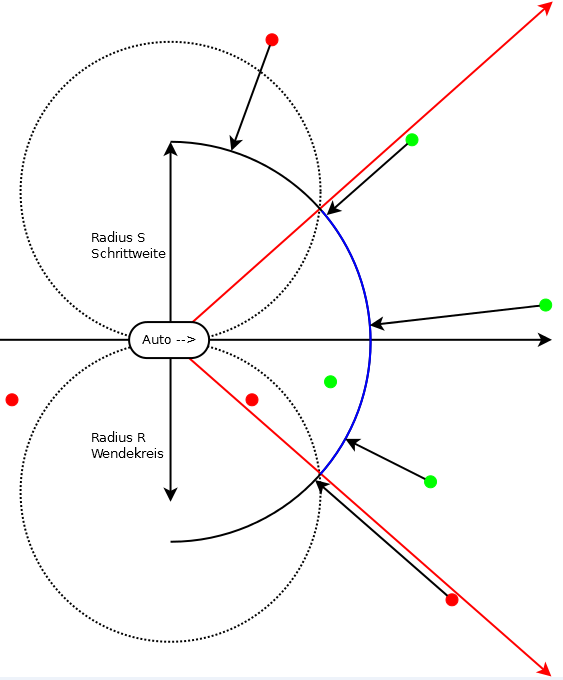
\includegraphics[scale=0.7]{Bilder/Projektion_der_Punkte.png} 
\caption{Projektion der Punkte auf Schrittweite}
\end{figure}
\subsubsection{Bestimmung des Vaterknotens}
Nachdem der Knoten an seinen nächsten Nachbarn projiziert wurde, wird nun aus allen nächsten Nachbar innerhalb eines Radius R der mit den besten Kosten gewählt. Im Verfahren zur Bestimmung des nächsten Nachbarn, siehe \ref{sec:Vorauswahl}, wurden die Punkte innerhalb der Schrittweite nicht berücksichtigt. Es ist dem Auto nicht möglich, vom Vaterknoten N zum Knoten K zu fahren, wenn K im Wendekreis des Autos liegt. \\
Für jeden Knoten im Radius R wird geprüft, ob dieser Knoten unseren neuen Knoten K erreichen kann. Das wird ausgerechnet, indem vom potentiellen Vaterknoten N aus zwei Mittelpunkte der Wendekreise bestimmt werden. Wenn der Abstand von K zu diesen Mittelpunkten kleiner ist als der Radius der Wendekreise, liegt K im Wendekreis und ist nicht erreichbar. Damit kommt N als Nachbar nicht in Frage. Falls kein nächster Nachbar im Radius R den Knoten K erreichen kann, wird K verworfen. \\
Nachdem erfolgreich ein Vaterknoten bestimmt und dem neu hinzugefügtem Knoten K zugewiesen wurde, muss noch die Ausrichtung oder Orientierung bestimmt werden, die das Auto im Knoten K hat.
\subsubsection{Bestimmung der Orientierung}

\begin{figure}
\label{fig:fig8}
\centering
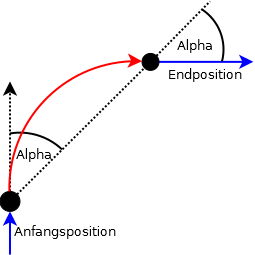
\includegraphics[scale=1]{Bilder/BerechnungOrientierung.png} 
\caption{Berechnung der Ausrichtung}
\end{figure}
Da das Auto im Vaterknoten N eine bestimmte Ausrichtung hat und mit nur einer Lenkeinstellung zum nächsten Knoten K gelangt, ist dort die Ausrichtung dadurch festgelegt und berechnet sich aus der Ausrichtung des Vaterknotens, Winkel $\theta$, und dem Richtungsvektor von N nach K. Der Richtungsvektor kann in einen Winkel relativ zu x-Achse mit Hilfe des Skalarprodukts ausgerechnet werden. Wie in der Zeichnung ~\ref{fig:fig8} zu sehen ist, wird der Winkel des Richtungsvektors zweimal auf die Ausrichtung im Vaterknoten addiert, um die Ausrichtung im neuen Knoten zu erhalten. \\

\subsection{Metrik und Kostenfunktion}
Eine besondere Bedeutung zur Erzeugung einer "guten" Trajektorie kommt der Kostenfunktion zu. Diese sorgt nicht nur dafür, welcher Knoten als Vaterknoten ausgewählt wird, sondern spielt auch beim Neuverknüpfen des Baumes eine Rolle.Somit kann mithilfe der Kostenfunktion für besonders gut abfahrbare oder besonders kurze Pfade gesorgt werden. \\
Da durch die Orientierung des Vaterknotens die Orientierung des Kindknotens bereits festgelegt ist (siehe Abbildung ~\ref{fig:fig8}, können aus eigentlich geraden Strecken sehr ungünstige Pfade entstehen.\\
 In Abbildung ~\ref{fig:fig5} wird als Kostenfunktion der euklidische Abstand benutzt. Knoten C wählt aus B1 und B2 den nächsten Nachbarn aus, das ist B2. Leider entsteht dadurch eine sehr kurvige Route, bei der vom fast maximalem Lenkeinschlag nach rechts auf den maximalen Lenkeinschlag der anderen Seite gewechselt werden muss. Neben Nachteilen des Komforts, der Sicherheit und längerem Weg wird auch die Ungenauigkeit höher. Anfangs wurde angenommen, dass der Lenkwinkel sich sofort ändern kann. Während bei kleinen Änderungen diese Annahme nur für kleine Fehler sorgt, sind die Auswirkungen bei solch starken Änderungen deutlicher spürbar.


\begin{figure}[htb]
  \label{fig:fig6}  
    \centering
    \begin{minipage}[t]{0.45\linewidth}
        \centering
        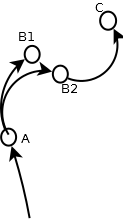
\includegraphics[width=.6\linewidth]{Bilder/B2Insert.png}
        \caption{einfache euklidischeKostenfunktion}
    \end{minipage}% <- sonst wird hier ein Leerzeichen eingefügt
    \hfill
    \begin{minipage}[t]{0.45\linewidth}
\label{fig:fig7}                 
        \centering
        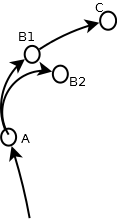
\includegraphics[width=.6\linewidth]{Bilder/B1Insert.png}
        \caption{erweiterte Kostenfunktion}
    \end{minipage}
\end{figure}


In Abbildung ~\ref{fig:fig7} hingegen wurde eine bessere Kostenfunktion gewählt, sodass über B1 gehend ein effizienterer, kürzerer Pfad entsteht. Die Kostenfunktion muss dabei die Ausrichtung des Autos beim Vaterknoten N berücksichtigen. [TODO Auswahl] Eine Möglichkeit wäre dann, die tatsächliche zu fahrende Strecke des Autos zu benutzen und dadurch effizientere Pfade zu bevorzugen. Eine andere Möglichkeit ist, zu harte Richtungsänderungen zu bestrafen und kleine $ \Delta \theta$ zu bevorzugen. \\
Als Lösung wurde hierbei eine Kombination aus dem euklidischem Abstand und der Winkeldifferenz der Knoten K und N zur Kostenberechnung zu benutzen. Die Kosten berechnen sich dann wie folgt: 
\begin{center}
$cost(K) = cost(N) +eukl. Abstand(K,N) * (1+Winkeldifferenz)$
\end{center} 
Bei einer geraden Strecke wird lediglich der euklidische Abstand als Kosten hinzuaddiert, bei einer Kehre von 180$^{\circ}$ das vierfache der euklidischen Kosten.  
\subsubsection{Rewiring}
[TODO Pseudo code] Der Knoten K wurde neu in den Baum hinzugefügt. Nun wird überprüft, ob bereits vorhandene Knoten besser erreichbar sind, wenn der Weg über K gewählt wird.
Dazu werden zunächst im Radius R alle in Frage kommenden Nachbarn ausgewählt. Aussortiert werden alle, die entweder vom Knoten K aus nicht erreichbar sind (gleiche Überprüfung wie oben) oder aber bei denen K keine Verbesserung bewirkt also die Kosten über den Knoten K gleich oder kleiner sind. \\
Wenn man von den jetzt noch ausgewählten Knoten M einfach K als Vater hinzufügen würde, müsste jeweils die Orientierung der Knoten, der Winkel $\theta$, geändert werden. Das Auto gelangt auf anderem Wege zu diesen Knoten und hat somit eine andere Ausrichtung als vorher. Allerdings kann es dadurch vorkommen, das wenn der Knoten $m \in M$ eine neue Orientierung hat, Kinder von m nicht mehr durch m erreichbar sind [TODO Zeichnung]. Deshalb wird, anstatt die Orientierung zu ändern, einfach ein neuer Knoten hinzugefügt, der zwar die gleicher Koordinaten hat wie m, aber eine andere Orientierung. Dies wird mit allen von K erreichbaren Knoten durchgeführt. Alle somit zum Baum neu hinzugefügten Knoten sind durch K besser erreichbar und können nun selbst zur Neuverknüpfung des Baumes beitragen. Somit wird der Algorithmus des Neuverknüpfens rekursiv auf alle im vorherigen Schritt durch das Rewiring neu hinzugefügten Knotens angewendet. \\
Der Vorteil dieses Mechanismus ist, dass mögliche Optimierungen schnell durch den Baum wandern und keine Knoten ungültig werden. Außerdem müssen nicht so viele randomisierte Punkte erzeut werden, was der Laufzeit zu Gute kommt. Nachteile sind allerdings eine geringere Anzahl von räumlich verteilten Punkten (es liegen Punkte "übereinander"). Zudem kann dieses Verfahren viel Zeit beanspruchen, ohne viel Effekt zu haben, wenn besonders viele Punkte im Baum existieren und Bereiche weit abseits der Zielregion neu verknüpft werden.


\subsection{Datenstruktur}
RRT* hat eine amortisierte Laufzeit von O(n log(n)). Um diese Laufzeit auch in der Praxis zu erreichen, muss auf spezielle Datenstrukturen zurückgegriffen werden. Insbesondere müssen mehrfach sowohl der nächste Knoten als auch die nächsten innerhalb eines Radius ermittelt werden. Für die sogenannte \textit{k-nearest neighbour} Suche und \textit{radius k-nearest neighbour} existieren bereits viele wissenschaftliche Untersuchungen und auch empfohlene Datenstrukturen, wie zum Beispiel k-d-Bäume \citep{Bentley75}. Leider benötigt der RRT* Algorithmus eine dynamische Datenstruktur, da Punkte erst nach und nach hinzugefügt werden. Eine weitere Einschränkung waren fehlende Implementierungen, die auf die Anwendungsfälle von RRT* zugeschnitten waren. \\
Aufgrund dieser Einschränkungen wurde keine komplizierte, unter Umständen bessere Datenstruktur gewählt. Stattdessen wurde ein einfaches Gitter implementiert, deren Achsen die x- und y-Werte des einzufügenden Punktes repräsentierte. Dadurch fallen Punkte, die nah beeinander sind, in die gleiche oder benachbarte Zellen. Je nach Wahl der Größe der Zellen müssen nur die Knoten der Zelle selbst und der Nachbarzellen überprüft werden. Ein weiterer Vorteil des Gitters ist das schnelle Einfügen eines Knotens: Dadurch dass das Gitter statisch bleibt können Arrays als Rahmen gewählt werden und die Laufzeit zum Einfügen von Knoten liegt bei O(1).\\
Solange allerdings noch sehr wenige Knoten sich im Gitter befinden, muss unter Umständen das gesamte Gitter nach Nachbarn abgesucht werden, was die Laufzeit stark verschlechtert. Innerhalb einer Zelle sind die Knoten in einer Liste gespeichert. Sollten sehr viele Knoten in eine Zelle fallen, dauert das Durchsuchen dieser Zelle sehr lange.



\subsection{Dokumentation der Durchführung und entstandener Artefakte}
[TODO] 
Anfangs wurde Python code programmiert. Dieser war weder objektorientiert noch besonders schnell, obwohl mit numpy eine für Vektorberechnungen optimierte Bibliothek benutzt wurde. Dann wurde - aufgrund von Performancegründen - zur Programmiersprache C++ gewechselt. Dabei wurde auch Objektorientierung eingeführt, um die einzelnen Knoten in ihrer Komplexität besser handhaben zu können. Dies verschlang sehr viel Zeit.\\
Als Datenstruktur wurde, sowohl eine Liste als auch ein Gitter verwendet. Zur Geschwindigkeitsoptimierungen wurde die Header-Bibliothek Eigen 3 benutzt. [TODO mehr schreiben wenn was funktioniert]
\subsection{Beschreibung besonderer Schwierigkeiten und wie diese umgangen wurden}
[TODO] evtl in nächstes/übernächstes kapitel. Lernfortschritte deutlich machen/ was habe ich aus den jeweiligen Problemen gelernt?

\subsubsection{Schwierigkeiten beim Einbinden bereits bestehender Architekturen}
 - Einbindung Eigen
 - Eclipse
 Erkenntnis, das eine mächtige Entwicklungsumgebung auch ein Stein am Fuß sein, mehr eine Behinderung als Hilfe wenn nicht richtig eingebunden, aber auch verweis auf zahlreiche vorteile (debuggen, schnell zwischen fkt hin und her springen)
 - visual Gps
 - fub controller
 
\subsubsection{Schwierigkeiten beim Programmieren und Kreieren eigener Strukturen}
- winkel und flüchtigkeitsfehler
- Programmieren in einer unbekannten programmiersprache, Zeiteinschätzungen
\subsubsection{Schwierigkeiten bei Tests und Übertragung auf das Auto}
	Hehe das kommt noch
\subsubsection{Tests und Testdatensätze/Szenarien für die Software)}
Test auf ....[TODO] wenns läuft...
\subsubsection{Korrektheitsbeweise}
\subsection{(Evaluation - nur wenn ich dafür Zeit habe)}
vllt rechtfertigung dass ich zu faul war/ nix geschafft habe??